\begin{enunciado}
 En $100$ lanzamientos de una moneda se observa $63$ caras y $37$ cruces.
 ¿Es una moneda balanceada?
 Utilice un nivel de significancia de $0.05$.
\end{enunciado}

\begin{solucion}
 Para la soluci\'on, se va a definir una variable aleatoria $X$,
 que es la cantidad de cruces que salen en $100$ tiros de la moneda,
 as\'{\i}, pues, probar que est\'a balanceado es equivalente
 a probar que $X$ sigue una distribuci\'on uniforme discreta
 $f(x;2) = \frac{x}{2}$ para $x\in{0,1}$.
 \begin{datos}
  $\phantom{0}$
  \begin{itemize}
   \item Tama\~no de la muestra: $n=100$.
   \item Frecuencias observadas:
   $O = \{ o_0 = 63, o_1 = 37 \}$.
   \item Probabilidades esperadas: $p_i = f(i;2)$,
   la funci\'on de probabilidad uniforme discreta con par\'ametro $k=2$,
   es decir $p_i = \frac{1}{2}, \forall i \in \{0,1\}$
   \item frecuencias esperadas:
   $E = \left\{ \left. e_i = n\cdot p_i = \frac{100}{2} = 50 \, \right| \, \forall i \in \{0,1\} \right\}$.
   \item Celdas totales del experimento: $k=2$.
   \item Grados de libertad de la prueba $\chi^2$: $v = k-1 = 1$.
  \end{itemize}
 \end{datos}

 \begin{hipotesis}
  Prueba de bondad de ajuste para probar $H_0:$
  que una variable aleatoria $X$ sigue una distribuci\'on uniforme
  $f(x;k) = f(x;2)$, para $x\in\{0,1\}$
  contra la alternativa $H_1$ de que no es as\'{\i}.
 \end{hipotesis}

 \begin{significancia}
  $\alpha = 0.05$.
 \end{significancia}

 \begin{region}
  De la tabla A.5 se tiene el valor cr\'{\i}tico
  $\chi^2_{\alpha,v} = \chi^2_{0.05,1} = 3.841$,
  por lo que la regi\'on de rechazo est\'a dado
  para $\chi^2 > 3.841$, donde
  $\chi^2 = \sum_{i=0}^{k-1} \frac{\left( o_i - e_i \right)^2}{e_i}$.
 \end{region}

 \begin{estadistico}
  \begin{eqnarray*}
   \chi^2 & = & \sum_{i=0}^{k-1} \frac{\left( o_i - e_i \right)^2}{e_i}
   =\frac{(63 - 50)^2}{50} + \frac{(37 - 50)^2}{50}
   = \frac{13^2 + 13^2}{50} = \frac{338}{50} \\
   & = & \frac{169}{25} = 6.76
  \end{eqnarray*}
 \end{estadistico}

 \begin{decision}
  Se rechaza $H_0$ a favor de $H_1$.
 \end{decision}

 \begin{conclusion}
  Hay suficiente evidencia para afirmar que la moneda no es legal.
 \end{conclusion}
 
 Finalmente, usando el archivo anexo
 \texttt{P15\_Prueba\_de\_bondad\_chi2\_01.r},
 que a su vez requiere los datos del archivo
 \texttt{DB16\_Problema\_080.csv}, con los siguientes cambios:
 \begin{verbatim}
> datos<-read.csv("DB16_Problema_080.csv",sep=";",encoding="UTF-8")
> varInteres<-"Frecuencia"
> varCelda<-"Lanzamiento.valor"
> distribucion<-1
> parametro_nombre<-NULL
> parametro_valor<-NULL
> combinar<-TRUE
> grafica<-TRUE
> tituloEjeX<-"Resultados al lanzar una moneda"
> alfa<-0.05
 \end{verbatim}
 \vspace{-0.7cm}
 el programa de R lanza el siguiente resultado:
 \begin{verbatim}
           Variable Distribución de ajuste Estadístico Chisq2 Grados de libertad
1 Lanzamiento.valor               Uniforme               6.76                  1
      Valor-p alpha Región de Rechazo                      Resultado
1 0.009322376  0.05       > 3.8414588 Se rechaza el ajuste de bondad
 \end{verbatim}
 \vspace{-0.7cm}
 que incluye la siguiente figura:
 \begin{center}
  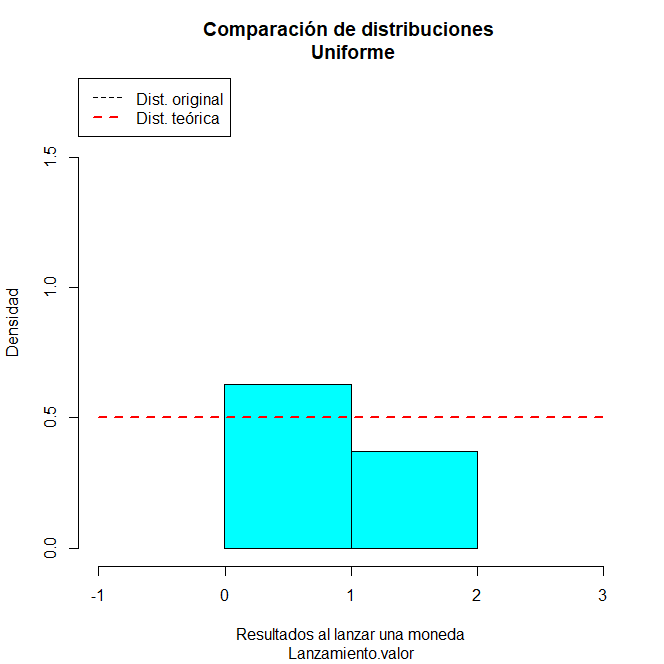
\includegraphics[scale=0.35]{Problema_80.png}
 \end{center}
 El cual coincide con los datos obtenidos,
 que es a lo que se quer\'{\i}a llegar.${}_{\blacksquare}$
\end{solucion}
